\chapter{Implementación de hardware}
En este capítulo se detallará cuál es el hardware utilizado para el desarrollo del sistema de acceso, se indicarán cuáles
son los requisitos mínimos que deben satisfacerse para que el sistema cumpla las características solicitadas, como
también se indicarán los sensores y equipos auxiliares usados junta con otras posibles opciones encontradas y las
razones por las que estas fueron descartadas.


\section{Estado actual del sistema de acceso por barreras}

\subsection{Sistemas tradicionales}

Hoy en día el sistema de uso de barreras para el control de ingreso y egreso a distintos recintos suelen generar molestias
en muchos de los usuarios, por la necesidad de realizar alguna acción extra, con esto nos referimos a la necesidad de
en muchas ocasiones de obtener y guardar algún tipo de ticket, este sistema lo vemos en la Fig. \ref{fig:sistema-tradicional}
que en caso de perderlo se tenga que pagar una multa económica, o bien de acercarse a un determinado lugar para poder realizar el pago por el tiempo de permanencia.

En este tipo de metodologías es donde queremos realizar un aporte a la reducción del impacto ecológico, ya que si se quita
la necesidad de imprimir uno o más tickets por cada vehículo que ingresa, se estaría disminuyendo considerablemente la
necesidad de utilizar papel y considerando que el método de impresión de estos tickets suele ser por impresión térmica,
proceso donde se utiliza un papel termosensible que al ser calentado se vuelve negro, que tiene un costo 
eléctrico adicional.
\begin{figure}
    \centering
    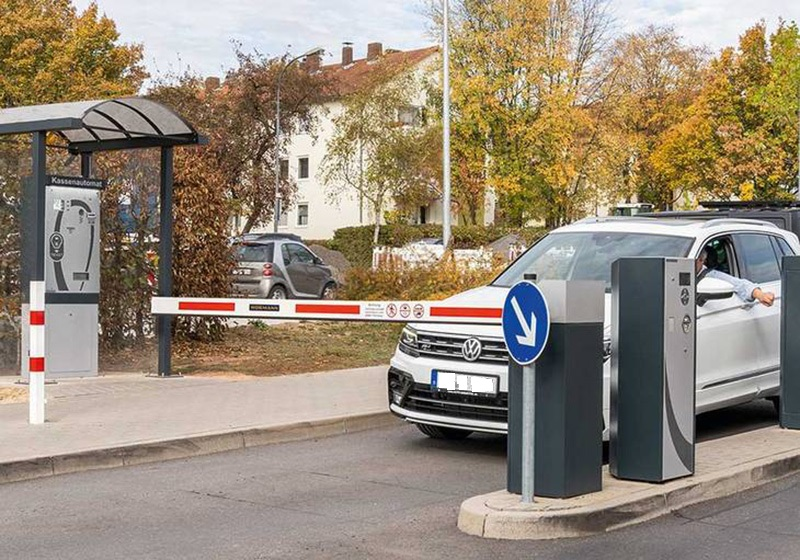
\includegraphics[width=0.5\textwidth]{imgs/sistema-control-acceso-barreras.jpg}
    \caption{Sistema tradicional de acceso por barreras por sistema de pulsador y ticket.}
    \label{fig:sistema-tradicional}
    %%https://www.aradock.es/nuevos-sistemas-de-control-de-accesos-barreras/
\end{figure}

Otro de los aspectos que destacan del uso actual del sistema de barreras en sistemas más manuales es la necesidad de
contar con  operarios trabajando en la barrera el tiempo que la barrera esté disponible, ya que en caso de no disponerlo
deberá quedar la barrera sin efecto, perdiendo por completo su utilidad.

\subsection{Sistemas Modernos}

Con el avance y el abaratamiento de los costos en la electrónica surgieron nuevos métodos que permitieron a los usuarios
prescindir de la necesidad de un ticket o una tercera persona que les facilite el acceso, el método principal es el uso
de controles remotos que al ser accionados, activan el mecanismo y abren el paso del vehículo.
 
Otro sistema que está ocupando gran parte del mercado en los últimos años es el que integra a la barrera un sistema de
RFID, que mediante la colocación de un emisor RF en el vehículo, Fig.\ref{fig:sistema-moderno} o por el método de tarjetas o monedas de proximidad y un
receptor en la barrera, al acercarse al ingreso se produce en el enlace que habilita o no al vehículo a ingresar.

\begin{figure}
    \centering
    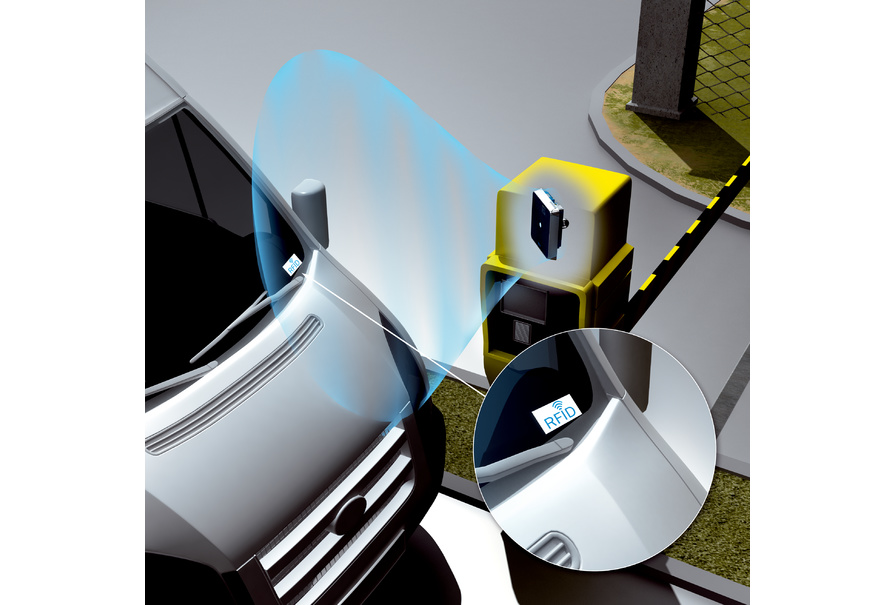
\includegraphics[width=0.8\textwidth]{imgs/sistema-control-acceso-barreras-rfid.jpg}
    \caption{Sistema moderno de acceso por barreras por sistema de RFID.}
    \label{fig:sistema-moderno}
    %%https://www.sick.com/mx/es/sectores/seguridad-de-los-edificios/seguridad-en-los-exteriores/control-de-acceso/acceso-sin-contacto-a-barreras-mediante-rfid/c/p360565
\end{figure}

Todos estos métodos son muy útiles y agilizan el tránsito por la zona de entrada que suele rondar entre los 15 y 20 segundos por
auto, pero también presentan la necesidad de contar con algún dispositivo o elemento externo para que este funcione, la finalidad
de este trabajo es obtener un método que reduzca el tiempo de ingreso lo máximo posible y retirar la necesidad de elementos
extras, es pocas palabras que solo con la proximidad del automóvil sea posible accionar la barrera.


Entonces ¿Qué requisitos debe tener el sistema para cumplir lo planteado?, en primera instancia y como el eje del trabajo
es utilizar un algoritmo de OCR, el hardware debe permitir el uso de una cámara de al menos una resolución de 480p, debe
soportar protocolos de comunicación (i2c,spi o UART) para el acople de sensores auxiliares necesarios, permitir conexión
Ethernet/wifi, soporte para el uso de Python 3.

\section{Selección de placas}
Teniendo en cuenta los requisitos mínimos planteados en la sección anterior, se presentan varias opciones posibles,
placas de la empresa Raspberry Pi, embebidos de la serie STM32 e incluso placas de la marca Arduino en sus versiones más
potentes, por nombrar las más conocidas. Aquí es donde nos surge el primero de los inconvenientes para tomar la decisión,
cuál sería la mejor opción que cumpla tanto las necesidades que debemos cubrir, como también que sea accesible para poder realizar las pruebas y testeos correspondientes.
Por lo que empezamos a investigar con qué variedad de placas contábamos y podíamos llegar a conseguir de manera sencilla,
y se tomo la decisión de quedarnos con 2 placas que decidimos llamar modelo SL y SL mini.

\subsection{Modelo SL mini}
La placa de la barrera SL mini es una Raspberry Pi 3 B+,Fig.\ref{fig:raspberry} la cual cuenta con un procesador
Broadcom BCM2837B0 y un Córtex A53 acompañado de 1 GB de RAM LPDDR2, lo cual es más que aceptable para correr un sistema operativo Raspberry Pi
OS(anteriormente conocido como Raspbian) basado en Debian(distribución de Linux), lo que era un requisito a cumplir desde
el comienzo del diseño del trabajo.

\begin{figure}
    \centering
    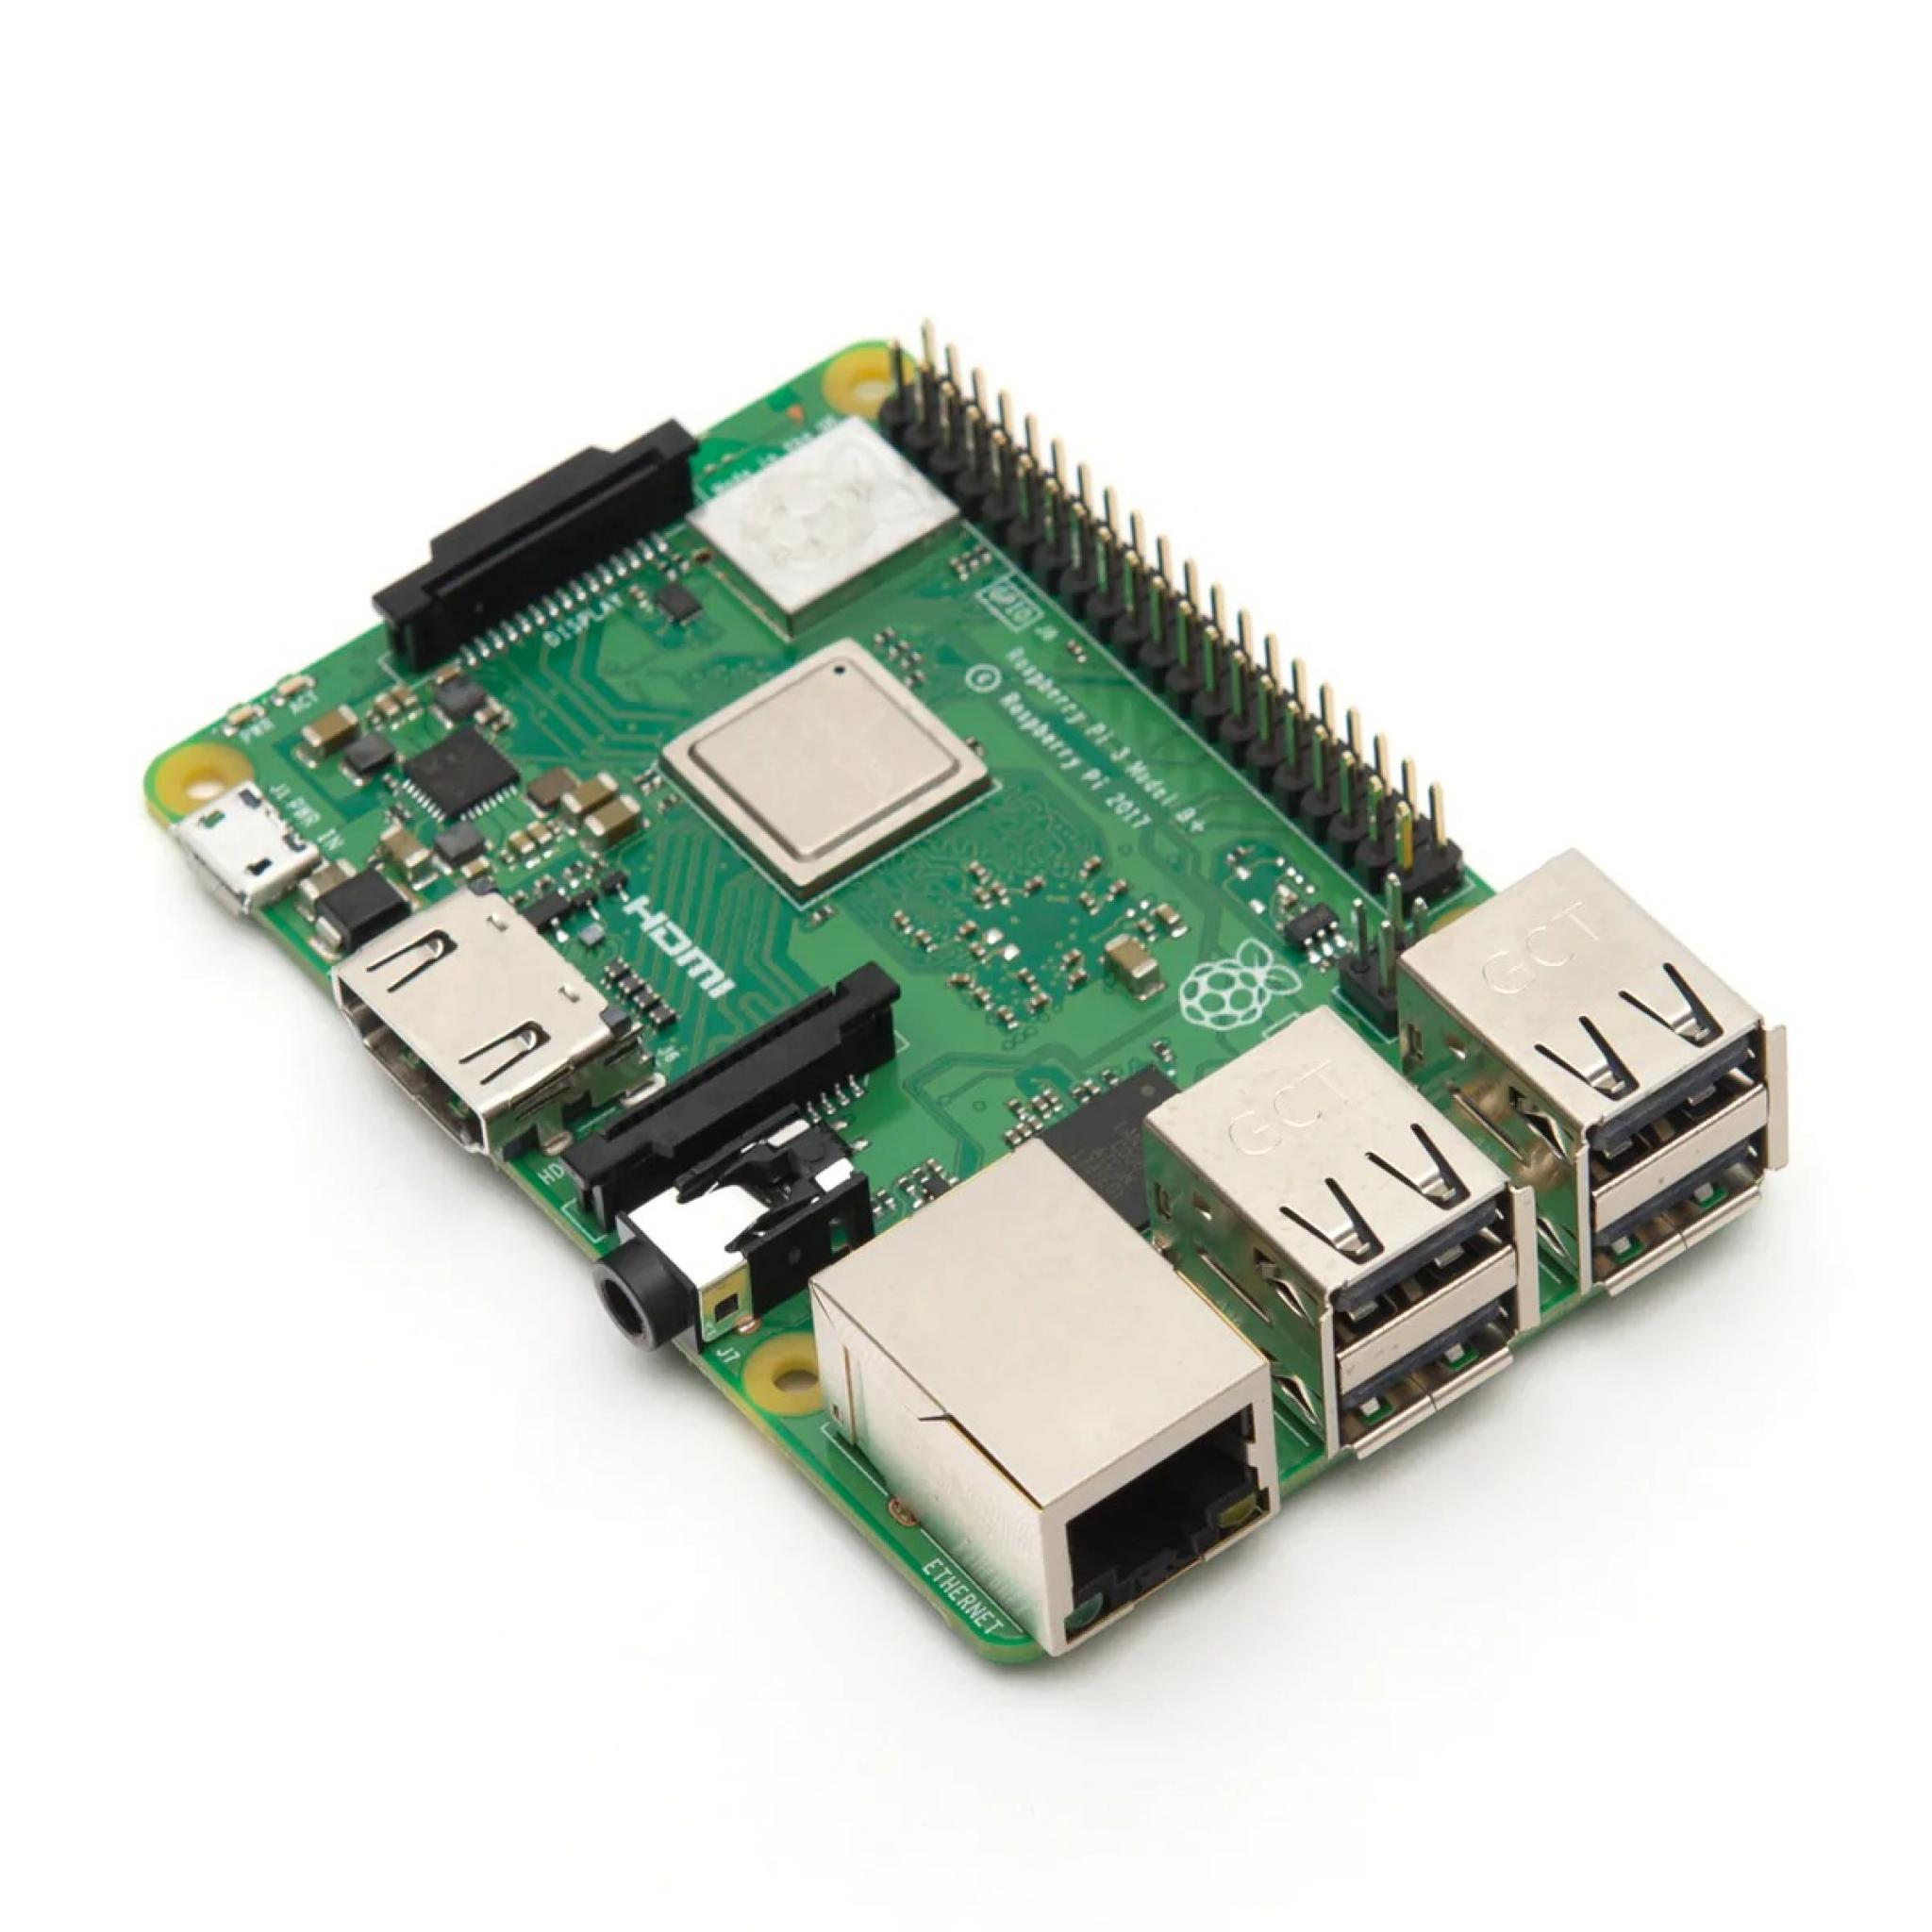
\includegraphics[width=0.8\textwidth]{imgs/Raspberry-pi3b+.jpg}
    \caption{Sistema embebido Raspberry Pi 3B+.}
    \label{fig:raspberry}
\end{figure}
Otro de los puntos importantes que destacan de la placa son los pines GPIO, pines de entrada/salida de propósito general
por sus siglas en inglés, lo que la hace sumamente sencilla a la hora de utilizarla junto a sensores comerciales.
La amplia conectividad integrada que posee fue un punto que la destacó sobre otras posibles placas de desarrollo, ya que
cuenta con puertos de conexión USB 2.0, puerto Gigabit Ethernet, conexión wifi 2,4 y 5,8 GHz y comunicación Bluetooth 4.2,
suple la necesidad de brindar conexión a internet de manera nativa sin necesidad de contar con periféricos extras que
puedan encarecer y obstaculizar el correcto funcionamiento del sistema.


La disponibilidad de la placa en el mercado, fue un punto importante que se consideró, ya que pensando en una futura
implementación del sistema a mediana o gran escala o la necesidad de cambio por rotura de la misma, podían dejar el
proyecto parado o inutilizado generando otros inconvenientes, además de que la placa es de nuestra propiedad, dándonos
completa disponibilidad para su uso.


Si bien las capacidades de la Raspberry son amplias, para este proyecto su poder de cómputo no fue suficiente para realizar
por sí misma el procesamiento de la imagen en un tiempo menor a 15 segundos, que es el tiempo promedio que se demora una persona
en ingresar a un recinto que cuenta con sistema de barrera en cualquiera de sus formas, demorando un aproximado de 1:30 
minutos, tiempo que se consideró excesivo.

\subsection{Modelo SL}
La placa de la barrera SL es una Nvidia Jetson TX1,Fig.\ref{fig:JTX1} la cual cuenta con un procesador Córtex A57, pero
cuenta con la característica de contar con núcleos de procesamiento de imagen, más específicamente posee 256 núcleos Nvidia Maxwell,
lo que la vuelve una opción excelente en lo que se refiere al trabajo con imágenes y videos, además su 4GB de RAM LPDDR4,
la hacen una opción mucho más potente en capacidad de cómputo que la Raspberry Pi 3 B+.


Para la realización del presente trabajo se contó con el kit de desarrollo provisto por la empresa Nvidia para el uso
del sistema embebido, en él se pueden encontrar todas las conexiones mencionadas en la barrera SL mini, lo que permite
el paso de los sensores de una placa a otra con suma facilidad.

\begin{figure}
    \centering
    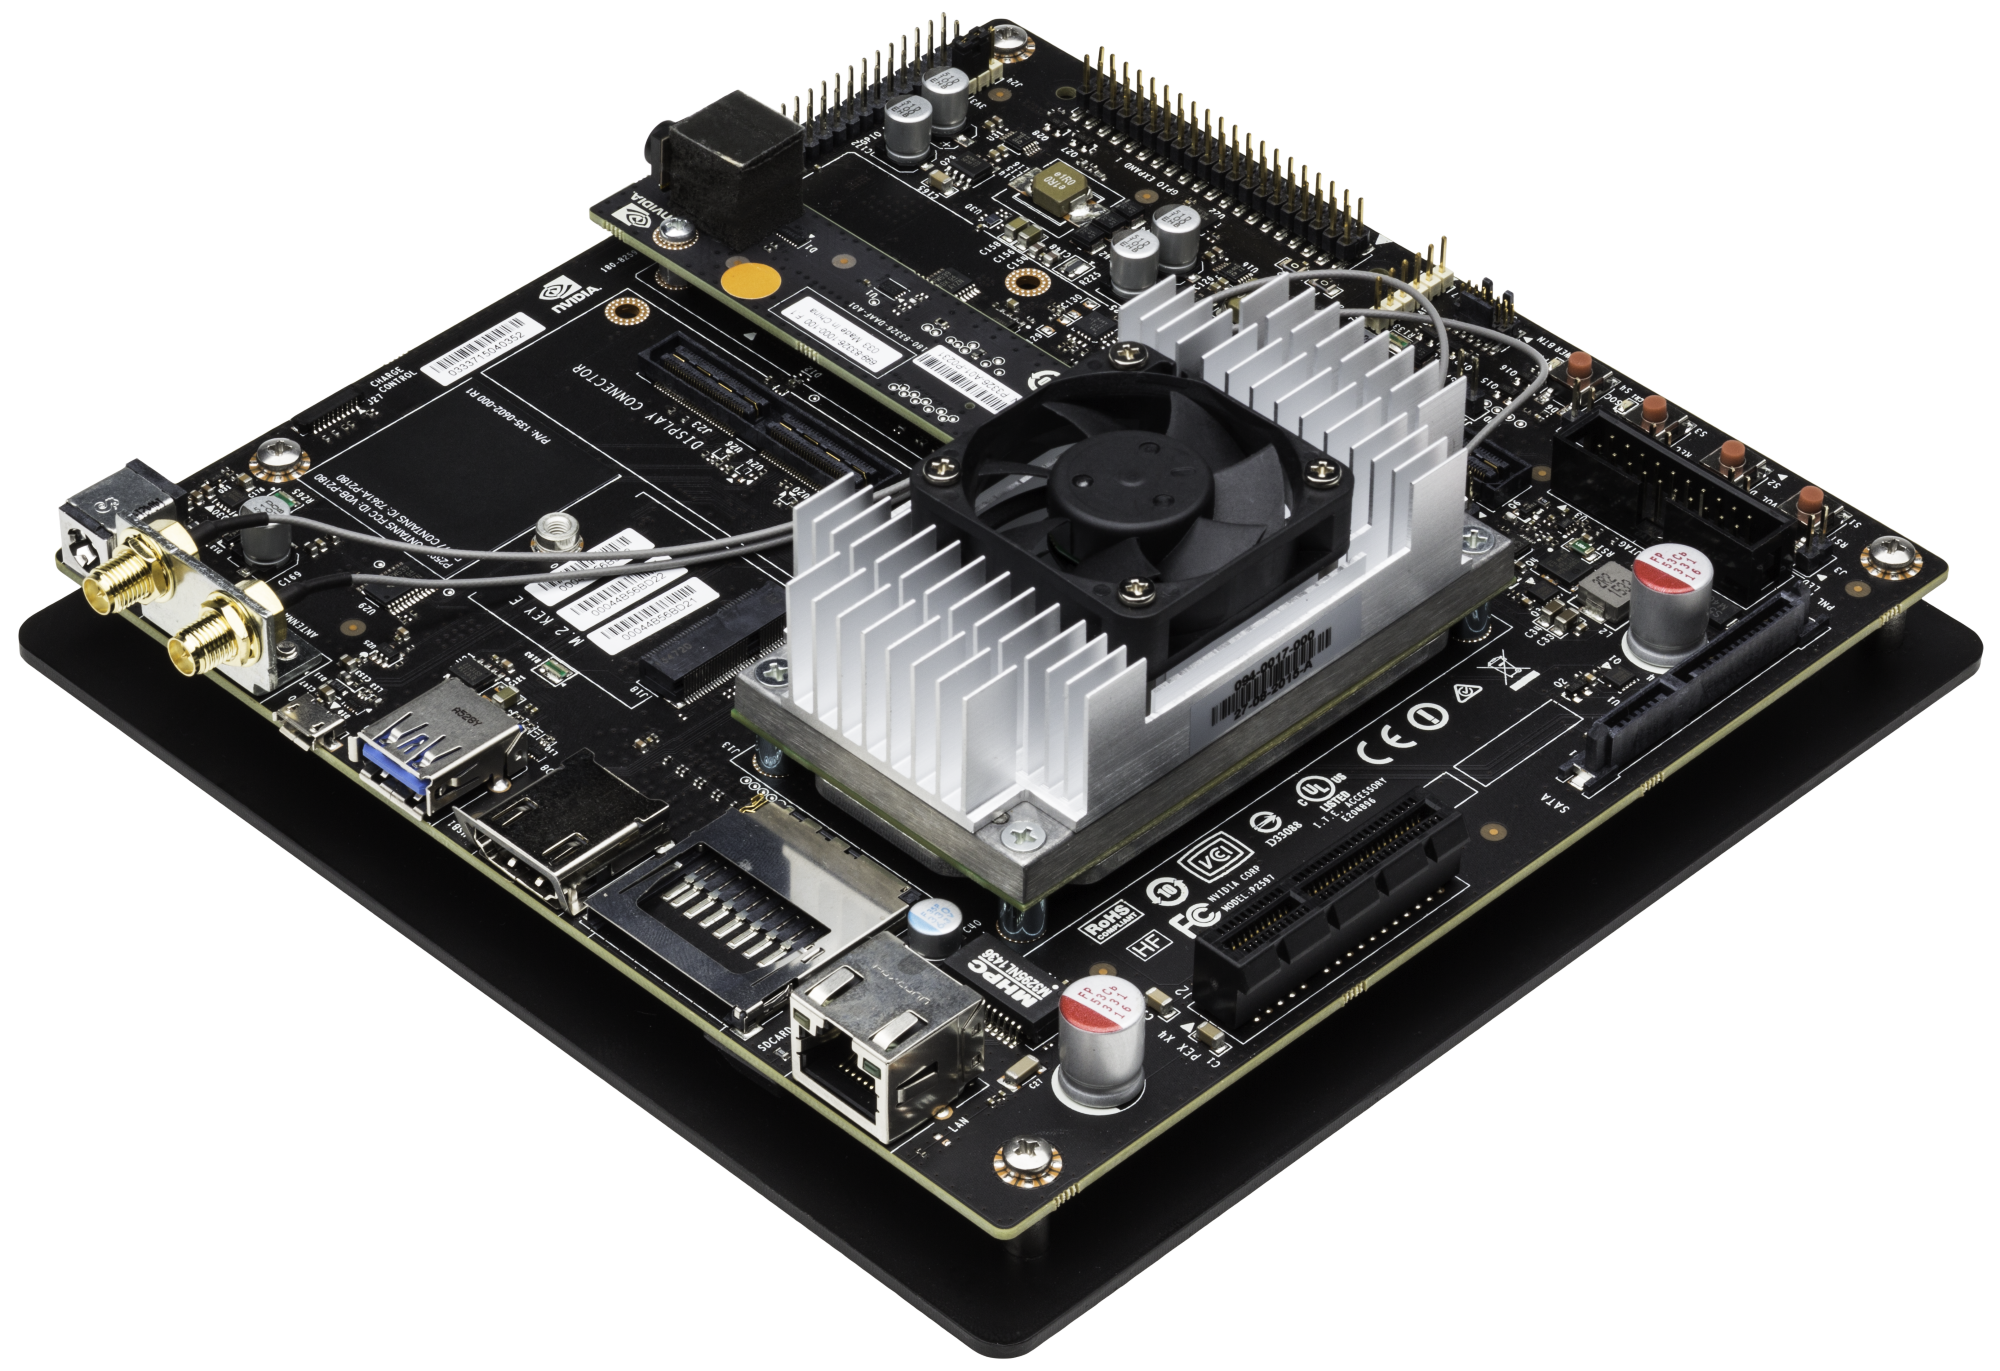
\includegraphics[width=0.8\textwidth]{imgs/JTX1-developerkit.png}
    \caption{Sistema embebido Nvidia Jetson TX1 developer kit.}
    \label{fig:JTX1}
\end{figure}
Este modelo de barrera cuenta con un sistema operativo JetPack 4.6.3 basado en Ubuntu 18.04(distribución de Linux) que 
como se hizo mención era requisito de diseño.
La disponibilidad de esta placa, es mucho menor respecto a la Raspberry, ya que presenta un costo mucho mayor 
A diferencia del modelo mini, el uso de la misma solo fue posible gracias a que nuestros tutores, la tienen disponible 
para su grupo de investigación y nos la facilitaron para usarla como favor.

En contra parte con el modelo mini, la placa del modelo SL está pensada para el trabajo con redes neuronales y el manejo 
de imágenes, por lo que es posible integrar todo el sistema de reconocimiento de caracteres dentro del mismo algoritmo embebido 
en la placa, teniendo un tiempo de respuesta de aproximadamente unos 6 segundos, tiempo más que aceptable para facilitar un rápido
acceso.

\section{Evaluación y selección de sensores}
Como se mencionó anteriormente fue necesario definir un actuador para saber cuando activar la cámara y tomar la imagen del vehículo 
para detectar su patente, por lo que nuevamente tuvimos que realizar un estudio de disponibilidad y costos de diversos sensores y cámaras que se 
encontraban disponibles en el mercado, además se buscó que el kit de cámara y sensor activador sea lo más portable entre los modelos SL y SL 
mini, para facilitar el cambio y evitar tener que modificar los códigos entre los modelos.
\subsection{Selección de cámara}
Si bien tanto el modelo de placa SL como su versión mini aceptan cámaras con conexionado propio provistas por las empresas que las crearon,
se tomó la decisión de utilizar una cámara web con conexión USB, Fig. \ref{fig:camara-usb}, se utilizó un modelo genérico, comprada vía Mercado 
Libre, ya que estas no requieren de drivers complementarios para funcionar, es decir son Plug and Play, son fácilmente reemplazables 
por otro modelo en caso de rotura o simplemente cambiarla por otra que sea de mejor resolución de imagen, además de poseer un precio reducido, 
comprada con otro tipo de cámaras USB u orientadas al uso en domótica.
\begin{figure}
    \centering
    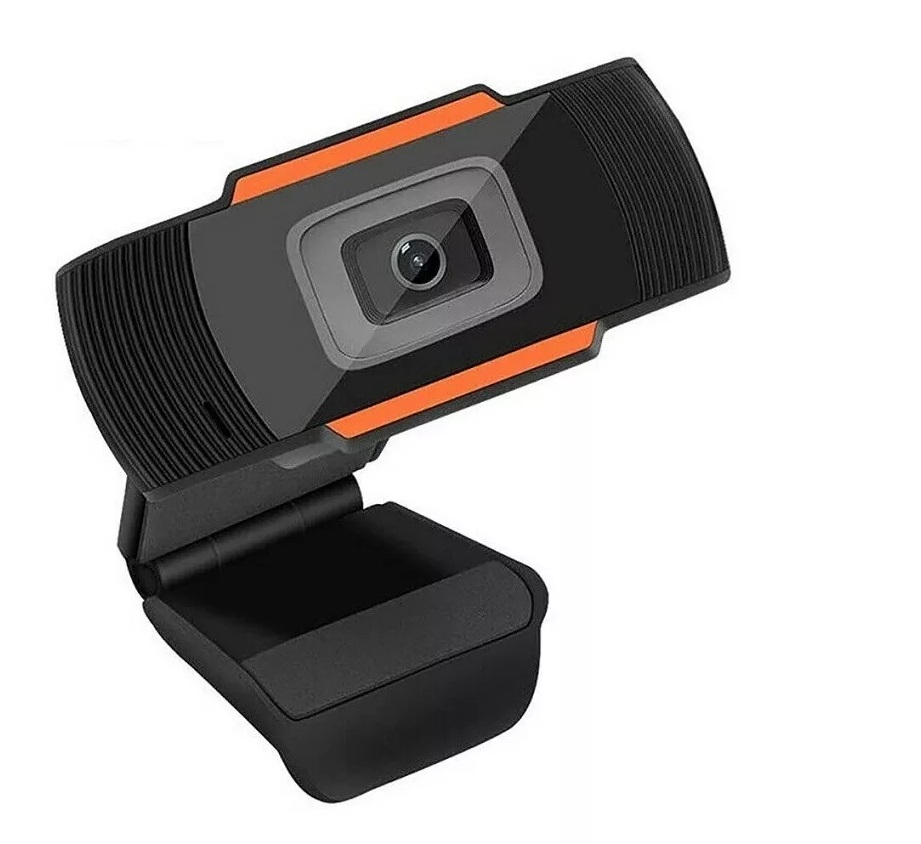
\includegraphics[width=0.5\textwidth]{imgs/camara-usb.jpg}
    \caption{Cámara utilizada para obtención de imágenes.}
    \label{fig:camara-usb}
    %https://www.mercadolibre.com.ar/camara-webcam-para-pc-microfono-usb-720p-hd-windows-10/p/MLA21775903#searchVariation=MLA21775903&position=2&search_layout=stack&type=product&tracking_id=8191aaa4-4b06-41e0-b681-ded2c4d4b641
\end{figure}

\subsection{Selección de activador}
Una vez que nos decidimos en la cámara, fue hora de analizar como decirle al sistema que obtenga la imagen, analizamos como suelen funcionar 
algunos sistemas que requieren que un objeto se aproxime o cruce un espacio específico y encontramos estas posibles opciones:

\begin{itemize}
\item Barrera infrarroja: mediante la utilización de un haz de luz infrarroja se indice sobre un receptor, por  lo cual al acercar el vehículo a
la barrera el haz se ve interrumpido generando un cambio en el receptor que accionaria la cámara. Este mecanismo cuenta con varios inconvenientes 
como la sensibilidad del receptor a la radiación infrarroja del ambiente, la posible interrupción del haz por suciedad (recordando que el 
sistema puede encontrarse a la intemperie), entre los  más destacados. Este método fue uno de los más probados por nosotros, en primera instancia
fabricamos una barrera infrarroja, pero no contaba con el alcance para permitir que un vehículo la atraviese, y las opciones comerciales, excedía
los costos que nos parecían razonables para invertir en este apartado. Por estas razones fue que el uso de una barrera infrarroja fue descartado.

\item Placa de presión: un sistema simple que usa una placa sobre el terreno que al ser pisada por el vehículo 
genera una señal de activación, el inconveniente se encuentra en la instalación de la plancha, debido a que no todos 
los accesos tienen la capacidad de permitirlo, por lo que esta opción se descartó.

\item Sensores capacitivos: estos generan campos magnéticos que en presencia de objetos se ven afectos, con lo 
que con una calibración correcta podría ajustarse para detectar vehículos, la difícil adquisición de los mismos por falta de stock, por costos o 
dificultad para crearlos llevaron a descartar esta opción.

\item Sensores ultrasónicos: Estos miden la distancia mediante la emisión de una onda ultrasónica por un transmisor y 
mediante el tiempo que tarda la onda emitida en llegar a un receptor se estima la distancia. Esta fue la opción elegida, ya que es una opción 
de un costo no muy elevado, relativa facilidad de integración a diversas placas embebidas y cuenta con la ventaja de tener una variedad de modelos
disponibles en el mercado que se adaptan a los diferentes protocolos de comunicación.
\end{itemize}
El sensor elegido para el diseño de ambos prototipos fue el sensor ultrasónico US-100,Fig. \ref{fig:sensor-US100}, el cual permite un 
rango de medición de 2 cm a 350 cm, compensado por temperatura, voltaje de alimentación entre 3V-5V y protocolo de 
comunicación UART. Por lo que es integrable a ambas placas por medio del puerto GPIO sin necesidad de requerir de conversores de nivel lógico 
ni hardware de alimentación adicional.
\begin{figure}
    \centering
    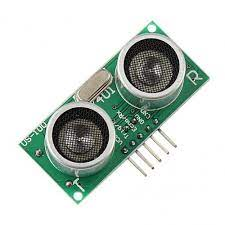
\includegraphics[width=0.5\textwidth]{imgs/us-100.jpg}
    \caption{Sensor US-100 usado en los prototipos.}
    \label{fig:sensor-US100}
\end{figure}

\section{Consumo energético}

El gasto energético es un punto que fue analizado, ya que, pensando en el uso racional de la energía, queríamos que nuestros prototipos no
presentaran un consumo excesivo, y que en un futuro si alguien lo deseaba sean alimentando por un panel solar junto con una batería.
Como la energía suministrada al conjunto cámara-sensor viene dada por las placas, solo se indicara el consumo requerido por las placas SL y SL mini.
\subsection{Consumo energético Modelo SL}

El requerimiento energético previsto por el fabricante para el kit de desarrollo de la Nvidia Jetson TX1 como se indica 
en el cargador que viene dentro del kit es de 19 volts y 4,74 ampers (máximo 90 Watts).

Lo que podría ser alimentado con el uso de una batería de 12 volts o 24 volts y un algún circuito externo que regule la 
tensión a los 19 volts solicitados, siempre y cuanto este sea capaz de suministrar la corriente necesaria.

\subsection{Consumo energético Modelo SL mini}

En el caso de la versión SL mini, tiene un consumo similar al de un cargador de celular moderno, es decir unos 5 volts y
2 ampers, ya que una corriente menor lleva a una notificación por parte de la placa, indicando que la energía no es la 
suficiente reduciendo la frecuencia de su procesador, ralentizando el equipo.

Este consumo reducido es fácilmente lograble con un sistema de carga de celular portátil, por lo que sería más sencillo 
alimentarlo en caso de no disponer una toma de corriente de la red doméstica.

\section{Diseño y ensamble}

Para la colocación del conjunto de prueba cámara-sensor, se diseñó e imprimió un contenedor en 3D,Fig. \ref{fig:contenedor-camara}
que sera soportado por un trípode o puede ser anclado a una pared o poste cercano a la zona de acceso.
\begin{figure}
    \centering
    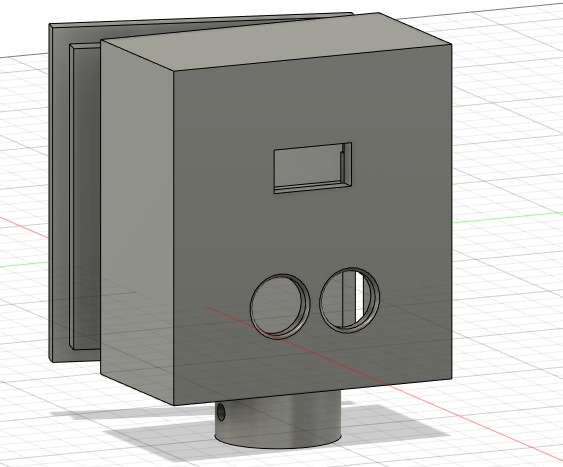
\includegraphics[width=0.5\textwidth]{imgs/contenedor-camara.png}
    \caption{Modelo 3D del contendor del paquete cámara-sensor.}
    \label{fig:contenedor-camara}
\end{figure}

Al tratarse de un prototipo se buscó que el diseño sea lo más simple posible, permitiendo ser fácilmente modificable, en el caso de necesitar
modificarlo en un futuro, ya sea por cambio de hardware o una necesidad de un punto de colocación diferente.

Se optó por colocar el sensor de proximidad en la zona inferior, ya que el ideal es colocar el contenedor a una altura de unos 60 cm 
aproximadamente, con lo que al tener el sensor en la zona baja se garantiza que la lectura que se tome sea de la trompa del automóvil y se 
obtenga un valor certero de la distancia.

Esto deja a la cámara en la zona superior del contendor dando una imagen lo más completa de la trompa del vehículo, tomando así la vista 
completa de la patente, esto con el fin de evitar que la patente salga recortada impidiendo que esta sea reconocida por el algoritmo.

Se dispuso un orificio en la zona inferior de la caja con la finalidad de colocar un eje, que permita la orientación del dispositivo, dependiendo 
el lugar donde se desee instalarlo, para la sujeción al eje se realizaron 2 pequeños orificios que permitan el paso de 2 tornillos que dejen fijo
el contenedor al eje.
\begin{figure}
    \centering
    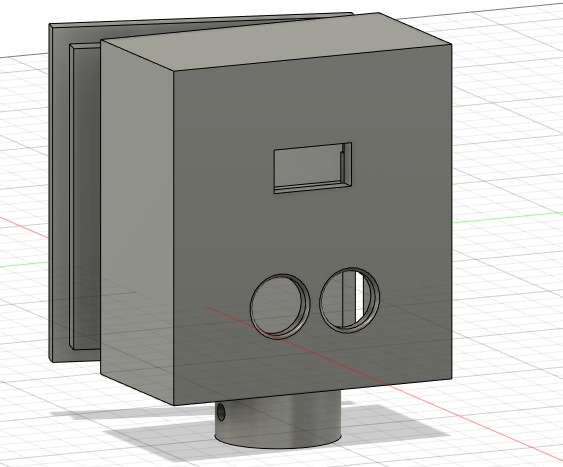
\includegraphics[width=0.5\textwidth]{imgs/contenedor-camara.png}
    \caption{sistema de sujeción del contenedor.}
    \label{fig:sujecion-contenedor}
\end{figure}

En la Fig. \ref{fig:contenedor-camara-real} se puede apreciar el contenedor ya con la camara y el sensor instalados.

\begin{figure}
    \centering
    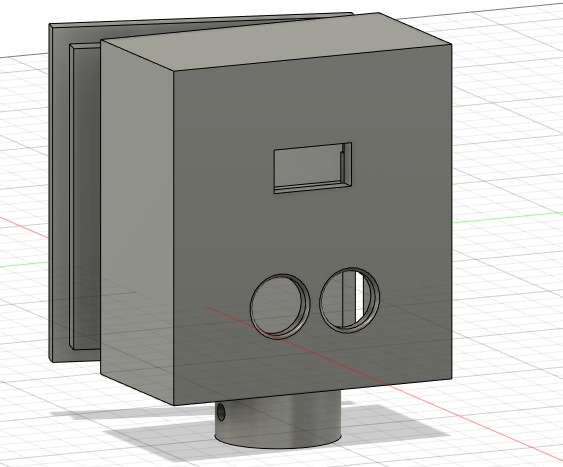
\includegraphics[width=0.5\textwidth]{imgs/contenedor-camara.png}
    \caption{Contendor del paquete cámara-sensor.}
    \label{fig:contenedor-camara-real}
\end{figure}

